\newpage

\section{Purchase Equipment}

\subsection{Parts List}
\begin{enumerate}[itemsep=-5pt]
\item Laptop with internet connectivity
\item Credit/Debit Card to Purchase items
\end{enumerate}

\subsection{Learning Objectives}
\begin{enumerate}[itemsep=-5pt]
\item Understand the world of microcontrollers
\item Learn about the Adafruit eco-system
\item Learn about the Circuit Playground Express/Bluefruit
\end{enumerate}

\subsection{CircuitPython Kit}

In this class you’re going to build some circuits that will enhance
your learning experience. Rather than just solving problems by hand
you’re going to take and analyze data. Over the summer of 2020, I
began to work with Tangibles that Teach and at the time they bundled
all components together. Unfortunately, that company has gone out of
business and as such for the time being you must build the kit
yourself. Here is a list of all the components in the kit

\begin{enumerate}[itemsep=-5pt]
\item Circuit Playground Bluefruit or Express + Included USB Cable
\item Micro Servo
\item Potentiometer
\item Photocell
\item Two Resistors (330 Ohm and 1K Ohm)
\item Alligator Clips x3
\item External Battery Pack
\item AAA Batteries x3
\item Breadboard
\item Push Button 
\item LEDs x2
\item Pitot Probe
\item LSM6DS33 + LIS3MDL - 9 DoF IMU (Optional)
\end{enumerate}

Below is also a photo of all the components listed above. When you get
your kit familiarize yourself with all of the components. I created
an \href{https://youtu.be/6sNNQrhnzLE}{unboxing video on Youtube} 
for you to take a look. The hardware kit is a collection of multiple
items. At the time of this writing the entire kit cannot be purchased
however the CircuitPlayground Express (CPX) can be purchased on
Adafruit\cite{AdafruitMAIN}. A photo of the kit is shown in the figure below. The photo shows the CPX on the left inside it's
protective zip lock bag.

\begin{figure}[H]
  \begin{center}
    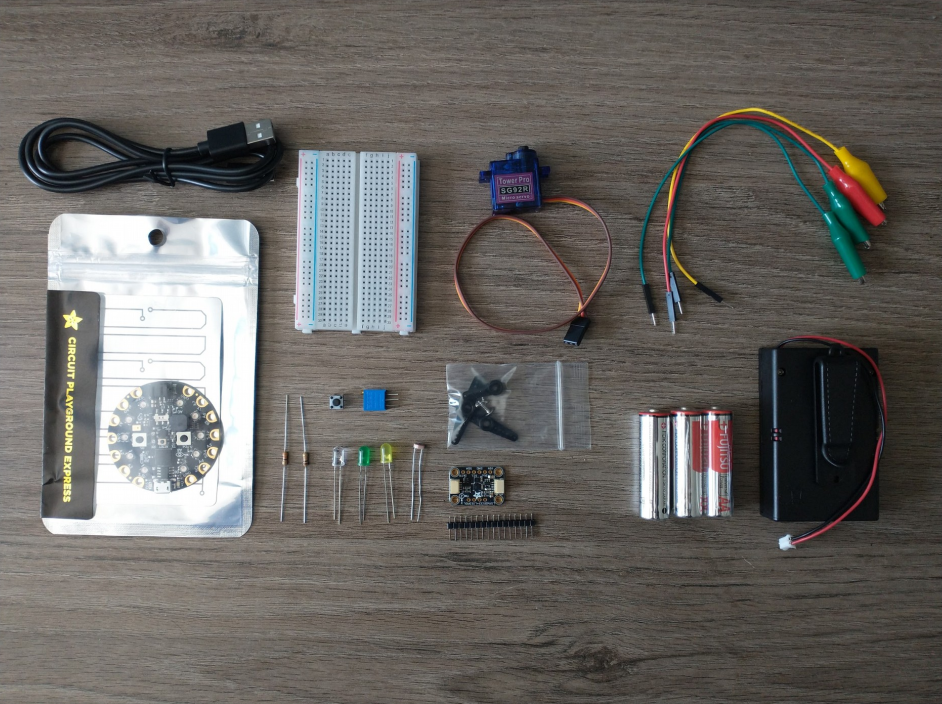
\includegraphics[width=0.8\textwidth]{Figures/components.png}
  \end{center}
\end{figure}

The CPX is a relatively new development board that operates in the
same style as Arduino\cite{Arduino}. That is, the student can
create a relatively simple script and then flash the software to the
CPX via USB. The Arduino operates in the same way. The benefit of the
CPX vs the Arduino is that the software is CircuitPython which is
indistinguishable from Python. As mentioned earlier, Python is in the
top 3 programming languages as stated by the Tiobe Index of
Programming\cite{Tiobe}. Other benefits include the components
built in to the CPX. The CPX itself contains a built in microphone,
accelerometer, light sensor, speaker, three push buttons, slide switch
and infrared sensor. The CircuitPlayground Express (CPX) also contains
10 smart NeoPixel LEDs and a ring of copper plated pads that can be
attached to the included alligator clips and breadboard. Students can
also elect to purchase the CircuitPlayground Bluefruit (CPB) which
does not have an infrared sensor but does contain bluetooth
functionality to send data wirelessly to the Adafruit Connect App
which runs on Apple/Android\cite{AdafruitBLE}.

\subsection{Assignment}
Your assignment for this module is to purchase the required equipment for your class. Note that the specific equipment will be instructor dependent so be sure you discuss with the instructor of your course before buying everything. At a minimum you must purchase a CPX or CPB but the rest of the items in your kit will depend on which modules your instructor wants you to do during the semester. {\bf Note that the CPX/CPB requires a microUSB cable and that cable must have a data line. Many USB cables are just power and ground.}

Once you've completed the project above, upload a PDF with all of the photos and text
below included. My recommendation is for you to create a Word document
and insert all the photos and text into the document. Then export the
Word document to a PDF. For videos I suggest uploading the videos to
Google Drive, turn on link sharing and include a link in your
PDF. Note that all code must be included in the appendix or you'll be
penalized 10\%. 


\begin{enumerate}[itemsep=-5pt]
\item A figure of your receipt of your purchases this semester (If you already own the CPX/CPB you may just take a photo of you holding the device) -60\%
\item Using the number of students in your class, compute the probability that at least one CPX/CPB will be shipped DOA (dead on arrival) assuming a failure rate of 1\%. - 20\%
\end{enumerate}

%\subsection{Quick Links}
%\begin{enumerate}[itemsep=-5pt]
%  \item \href{https://www.tangiblesthatteach.com/product-page/instrumentation-kit-for-me-316}{Kit}
%  \item \href{https://a2279211-28c1-4f46-9477-0d3265900c7f.filesusr.com/ugd/2413aa_ca39175b0a514b838ec96893b90590eb.pdf}{Document}
%  \item \href{https://youtu.be/6sNNQrhnzLE}{Unboxing Video}
%\end{enumerate}
%\subsection{Turning in this assignment}
%\begin{enumerate}[itemsep=-5pt]
%  \item Upload a receipt of ALL of your purchases - 50\%
%  \item Put your name and the names of your group members. If working
%    alone, tell me you are planning on working alone in the PDF you
%    upload. In times of COVID, everyone is working alone - 50\%
%\end{enumerate}
%% \newpage

%% \begin{center}\LARGE{ONLY READ BELOW IF YOU DON’T WANT TO BUY THE KIT
%%     ABOVE}\end{center}

%% \subsection{Purchase Items Yourself}

%% The bill of materials listed below is designed for 2 or 4 students to work together and share
%% pieces. This kit is not optimized for 3 students. If you are a remote/online student or you just
%% prefer to work alone then you have the option of purchasing everything yourself. The cost per
%% student in a group of 4 and 2 is listed as well as the cost if working alone. You’ll find that even
%% with the optional equipment, the cost of working alone is still less than the price of a standard
%% college textbook. Note that if you are working alone, be sure to only purchase 1 of each item. If
%% working in pairs you also have the option of purchasing one of each item. Finally, if you own
%% some of these components you may wish to simply purchase each item separately. A detailed
%% parts breakdown is shown after the rubric.

%% \subsection{Bill of Materials (per 4 students)}

%% \begin{figure}[H]
%%   \begin{center}
%%     \begin{tabular}{|l|c|c|}
%%       \hline
%%       Item (ONLY IF YOU DON’T WANT THE KIT ABOVE) & Quantity & Total
%%       Cost \\
%%       \hline
%%       \href{https://www.adafruit.com/product/3333}{Circuit Playground Express (CPX)} & 2 & \$50 \\
%%       \hline
%%       \href{https://www.adafruit.com/product/169}{Servo} & 2 & \$10 \\
%%       \hline
%%       \href{https://www.adafruit.com/product/592}{USB Cable} & 2 & \$6 \\
%%       \hline
%%       \href{https://www.amazon.com/Smraza-Breadboard-Resistors-Mega2560-Raspberry/dp/B01HRR7EBG/ref=sr_1_3?dchild=1&keywords=photocell+circuit+kit&qid=1590531716&sr=8-3}{Electronics Kit} (Photocells, Resistors, Trimpot) & 1 & \$13 \\
%%       \hline
%%       \href{https://www.amazon.com/WGGE-WG-026-Pieces-Colors-Alligator/dp/B06XX25HFX/ref=sr_1_1_sspa?dchild=1&keywords=alligator+clips&qid=1613147431&sr=8-1-spons&psc=1&spLa=ZW5jcnlwdGVkUXVhbGlmaWVyPUFLRjlYRVM3SDIySVAmZW5jcnlwdGVkSWQ9QTAwNDczMzEyODNCVTJWSjlMR0NEJmVuY3J5cHRlZEFkSWQ9QTAwMDQyMjkzSlJLNjJRWk9CSVZEJndpZGdldE5hbWU9c3BfYXRmJmFjdGlvbj1jbGlja1JlZGlyZWN0JmRvTm90TG9nQ2xpY2s9dHJ1ZQ==}{Alligator Clips} & 1 & \$4 \\
%%       \hline
%%       {\bf Total} & & {\bf \$83} \\
%%       \hline
%%       {\bf Cost per student in a group of 4} & & {\bf \$21} \\
%%       \hline
%%       {\bf Cost per student in a group of 2} & & {\bf \$25} \\
%%       \hline
%%       {\bf Cost if working alone} & & {\bf \$50} \\
%%       \hline
%%        & & \\
%%       \hline
%%       {\bf Optional Equipment} & & \\
%%       \hline
%%       \href{https://www.adafruit.com/product/3287}{External Power Supply} & 2 & \$6 \\
%%       \hline
%%       \href{https://www.adafruit.com/product/3349}{AA Batteries} & 2 & \$6 \\
%%       \hline
%%       \href{https://www.amazon.com/Hobbypower-Airspeed-MPXV7002DP-Differential-controller/dp/B00WSFWO36/ref=sr_1_3?dchild=1&keywords=Airspeed+sensor+kit&qid=1590532161&sr=8-3}{Analog Pitot Probe} & 1 & \$31 \\
%%       \hline
%%       \href{https://www.adafruit.com/product/4485}{Rate Gyro (LSM6D3SS)} & 1 & \$10 \\
%%       \hline
%%       & & \\
%%       \hline
%%       {\bf Total with Optional Equipment} & & {\bf \$136} \\
%%       \hline
%%       {\bf Cost per student in a group of 4} & & {\bf \$34} \\
%%       \hline
%%       {\bf Cost per student in a group of 2} & & {\bf \$50} \\
%%       \hline
%%       {\bf Cost if working alone} & & {\bf \$97} \\
%%       \hline
%%     \end{tabular}
%%   \end{center}
%% \end{figure}

%% \subsection{Detailed Parts List}

%% If you want to just purchase each component separately you can, just
%% make sure you have all of the parts below.

%% \begin{enumerate}[itemsep=-5pt]
%%   \item Circuit Playground Express (CPX)
%%   \item Servo
%%   \item Alligator Clips
%%   \item USB Cable
%%   \item Push Button
%%   \item Breadboard
%%   \item Photocell
%%   \item Resistors (10 kOhm, 330 Ohm, 1 kOhm)
%%   \item LED (x3 in case you fry one)
%%   \item Male to Male Wires (x2)
%%   \item Potentiometer
%% \end{enumerate}

%% You can also purchase some optional equipment as shown below.

%% \begin{enumerate}[itemsep=-5pt]
%% \item Rate Gyro (LSM6D3SS)
%% \item Male to Male Wires (x2)
%% \item Alligator Clips (x1)
%% \item Double Sided Tape
%% \item Analog Pitot Probe
%% \end{enumerate}